\documentclass{article}

% NeurIPS-style packages
\usepackage[utf8]{inputenc}
\usepackage[T1]{fontenc}
\usepackage{hyperref}
\usepackage{url}
\usepackage{booktabs}
\usepackage{amsfonts}
\usepackage{amsmath}
\usepackage{nicefrac}
\usepackage[protrusion=true,expansion=false]{microtype}
\usepackage{graphicx}
\usepackage{multirow}
\usepackage{array}
\usepackage{xcolor}
\usepackage{geometry}
\usepackage{setspace}

\geometry{
  a4paper,
  top=2.5cm,
  bottom=2.5cm,
  left=2.5cm,
  right=2.5cm
}

\graphicspath{{../../reports/results/}}

\title{
  Modeling Divergence Between Community-Perceived and\\
  Automatically Calculated MTG Commander Brackets
}

\author{
  Henrique Bidarte Massuquetti \and Marco Antônio Chitolina da Silva
}

\date{}

\begin{document}

\maketitle

% ============================================================
\begin{abstract}
% ============================================================

Commander is the most popular casual format of \textit{Magic: The Gathering} (MTG). Before each game, players label their decks on a five-level power scale called the Commander Brackets, but the assignment is subjective and varies between playgroups. Automated calculators read the same deck and return a bracket from a fixed rule set; the two readings often disagree. We study this disagreement on 12{,}135 public Commander decks collected from Archidekt, each carrying a community-assigned bracket \(y_{\text{com}}\) and a calculator-assigned bracket \(y_{\text{calc}}\) in \(\{2,3,4\}\). Each deck is encoded in two ways: a sparse Bag of Cards (BC) over the card vocabulary and a dense Deck Features (DF) vector of 114 structural attributes. We train six classifiers on each representation to predict \(y_{\text{com}}\) under nested cross-validation, and compare their out-of-fold predictions to \(y_{\text{calc}}\). We do not treat either source as ground truth: the goal is to measure the misalignment between two imperfect readings of the same construct and to identify which deck-level signals drive each side of it.

\end{abstract}

% ============================================================
\section{Introduction}
\label{sec:intro}
% ============================================================

A Commander game is fun when the four decks at the table sit close to each other in power. Pairings drift quickly: a deck that is slightly faster, slightly more consistent, or carries one or two cards that close the game on their own can flatten the experience for the other three players. The format does not enforce any of this --- it leaves the negotiation to the players, before the game starts.

To make that negotiation easier, the Commander community converged on a small shared vocabulary. The format's official committee published a five-level system, the Commander Brackets, where each player labels their own deck. The label is largely subjective: it carries a few hard caps on specific cards but otherwise reflects the player's reading of their own deck. Two players with similar decks routinely pick different brackets, and the same player may pick different brackets for the same deck on different days.

In parallel, the community built automated calculators that read a decklist and return a bracket from a deterministic rule set. The calculators are not subjective --- they see only the cards --- but they encode their own assumptions about what makes a deck strong. The two readings disagree, and the disagreement is itself the object of study.

We collect 12{,}135 public Commander decks from Archidekt, each carrying a community bracket \(y_{\text{com}}\) and a calculator bracket \(y_{\text{calc}}\) from EDHPowerLevel, both in \(\{2,3,4\}\). We encode each deck as a sparse Bag of Cards (BC) and as a dense Deck Features (DF) vector, train six classifiers on each representation to predict \(y_{\text{com}}\), and compare the out-of-fold predictions against \(y_{\text{calc}}\). Figure~\ref{fig:overview} sketches the pipeline on a single deck.

\begin{figure}[h]
\centering
% TODO: replace this placeholder with a composite figure built from a real
% deck in the dataset. It should show (i) the Archidekt decklist, with arrows
% pointing to (ii) the deck's BC row (sparse card-count vector) and (iii) the
% deck's DF row (dense structural vector), plus (iv) a table comparing its
% y_com and y_calc, with the deck framed inside one nested-CV training fold.
\fbox{\parbox{0.95\linewidth}{\centering\vspace{1.5cm}\textit{[Figure placeholder]} An Archidekt deck is projected into the BC (sparse card-count row) and DF (dense structural row) representations and labeled with both \(y_{\text{com}}\) and \(y_{\text{calc}}\). The same deck is placed inside one outer training fold of the nested cross-validation.\vspace{1.5cm}}}
\caption{Overview of the pipeline. One Archidekt deck $\rightarrow$ two representations $\rightarrow$ two labels $\rightarrow$ one fold of nested CV.}
\label{fig:overview}
\end{figure}

\paragraph{Research question.} \textit{To what extent do Archidekt-assigned Commander brackets diverge from automatically calculated bracket estimates, and which deck characteristics explain the disagreement?}

\paragraph{Contributions.}
\begin{enumerate}
  \item A curated dataset of 12{,}135 high-visibility Commander decks with both \(y_{\text{com}}\) and \(y_{\text{calc}}\) labels in \(\{2,3,4\}\), released along with extraction code.
  \item A direct measurement of the raw divergence between \(y_{\text{com}}\) and \(y_{\text{calc}}\) on the modeling set, including signed distribution and structural correlates.
  \item Two complementary deck representations (BC and DF) compared across six classifiers under nested cross-validation, with strictly per-fold preprocessing.
  \item A model-level divergence analysis that asks which representations and which signals drive each side of the disagreement.
\end{enumerate}

\paragraph{Outline.} Section~\ref{sec:background} reviews Magic, Commander, and the two power-assessment systems we use. Section~\ref{sec:dataset} documents the data, the EDA, and the two deck representations. Section~\ref{sec:spotcheck} describes the spot-checking pass that selects the algorithm pool. Section~\ref{sec:training} describes nested cross-validation and reports model results. Section~\ref{sec:discussion} discusses limitations. Section~\ref{sec:conclusion} concludes. Appendices provide MTG background, an extended preprocessing rationale, the full DF feature catalog, and the full spot-checking table.

% ============================================================
\section{Background}
\label{sec:background}
% ============================================================

This section gives the minimum context needed to read the rest of the paper. Game terminology used later (Game Changers, tutors, combos, EDHREC rank, salt score, layouts, keywords) is defined in Appendix~\ref{app:mtg}. A walkthrough of how a turn of Commander is played sits in Appendix~\ref{app:mtg:turn}.

\subsection{Magic: The Gathering}
\label{sec:bg:mtg}

MTG is a turn-based collectible card game first published in 1993.\footnote{\url{https://magic.wizards.com}} A player builds a deck from a pool of tens of thousands of unique cards, draws a hand, and casts spells using a resource called \textit{mana}. Each card has a type --- creature, instant, sorcery, artifact, enchantment, planeswalker, or land --- and a converted mana cost (CMC) that says how much mana is needed to play it. Lands produce mana; everything else consumes it.

The game has many formats. Each defines deck-construction rules, the legal pool of cards, and the number of players at the table. Our work is restricted to one format, Commander.

\subsection{Commander}
\label{sec:bg:commander}

Commander, also known as EDH, is the format we study. A deck has exactly 100 cards. One card is the \textit{commander}: a legendary creature that begins in a separate zone and can be cast at will throughout the game. The remaining 99 cards must respect the commander's color identity --- the set of mana colors appearing in its cost and rules text. With the exception of basic lands, each card may appear at most once (the \textit{singleton} rule).

A default Commander game has four players, each playing their own deck and starting with 40 life. Games are longer than in two-player formats and reward decks that scale into the late game. Because each player brings a different deck, the four-way table can have a much wider spread of strategies and speeds than a two-player match.

\subsection{Why power balance matters}
\label{sec:bg:power}

A Commander table works when the four decks land in a comparable range of power. When one deck is noticeably faster, more consistent, or includes a few cards that end the game on their own, the experience for the other three players degrades. The format does not enforce balance: it leaves the players to negotiate it before the game starts.

The metrics that the community has converged on are not deck win rates, but rather signals tied to deck \textit{structure}: how many \textit{Game Changers} a deck plays, how many \textit{tutors}, how many \textit{two-card combos}, the mana curve, and the rough cost of the deck. These are the same signals the automated calculators count, and they are the signals our DF representation captures.

\subsection{Commander Brackets (community label \(y_{\text{com}}\))}
\label{sec:bg:brackets}

The format's official committee published a five-level bracket system in October 2024. Bracket~1 is casual and thematic; bracket~5 is cEDH (competitive EDH). The middle brackets, 2--4, cover most casual play. Each bracket has a few hard caps --- for instance, on the count of Game Changer cards --- but most of the label is left to the player's reading of their own deck.

In our dataset, \(y_{\text{com}}\) is the bracket the deck creator selected on Archidekt,\footnote{\url{https://archidekt.com}} the deck-building platform we scraped. It carries the same kind of noise as any self-report: a well-tuned deck without any Game Changers can be stronger than a poorly-built deck that happens to include several, and two players with similar decks may still pick different brackets.

\subsection{Automated calculators (calculator label \(y_{\text{calc}}\))}
\label{sec:bg:calculator}

Several community tools take a decklist as input and return a bracket from a deterministic rule set. We use EDHPowerLevel.\footnote{\url{https://www.edhpowerlevel.com}} The calculator counts cards in named lists (Game Changers, tutors, extra-turn effects, mass land denial), counts known combo pieces, and weighs in card price and EDHREC\footnote{\url{https://edhrec.com}} popularity. It does not see the player; it only sees the cards. The bracket it returns is deterministic given the inputs, but the inputs change over time --- card prices and EDHREC ranks move daily.

The two readings disagree. A deck the player called bracket~3 may receive a calculator bracket of 2 or 4, and the rate of disagreement is large enough to motivate this work. Neither label is correct: \(y_{\text{com}}\) reflects the player's reading, \(y_{\text{calc}}\) reflects one rule set. The aim of this paper is to characterize the misalignment, not to arbitrate it.

% ============================================================
\section{Dataset Construction}
\label{sec:dataset}
% ============================================================

\subsection{Data sources}
\label{sec:data:sources}

The community labels come from \textbf{Archidekt}, a public deck-building platform that stores user-created decklists, view counts, and the user-assigned bracket. Archidekt exposes a paginated REST API that we used to collect raw deck payloads, including the full mainboard and metadata.

The calculator labels come from \textbf{EDHPowerLevel}, a browser-based calculator that takes a pasted decklist and returns a bracket assignment and a continuous power score. EDHPowerLevel does not expose a programmatic API. We automated the interface with a headless Chromium browser driven by Playwright, pasting each decklist and reading the rendered bracket from the DOM.

\subsection{Extraction pipeline}
\label{sec:data:extraction}

Collection retrieved 14{,}421 deck records from the Archidekt API across the brackets we queried. We removed 1{,}467 duplicate deck IDs (the same deck listed under multiple paginated queries) and 4 deck records that produced identical card-list fingerprints, leaving 12{,}950 unique decks. Each remaining deck was then sent to EDHPowerLevel to obtain \(y_{\text{calc}}\) and the auxiliary power score.

Every deck we retained on the Archidekt side satisfied, by construction of the API query:
\begin{itemize}
  \item Public deck on Archidekt, format Commander;
  \item User-assigned bracket \(y_{\text{com}} \in \{2,3,4\}\);
  \item At least 1{,}000 views on Archidekt;
  \item Exactly 100 cards in the mainboard;
  \item Mainboard only --- maybeboard, sideboard, tokens, and extras were ignored.
\end{itemize}

After joining \(y_{\text{calc}}\), 815 decks (6.3\%) received \(y_{\text{calc}} \in \{1,5\}\) and were dropped from the supervised setup, since brackets~1 and~5 are sparsely populated extremes. This yields the \textbf{modeling set of 12{,}135 decks}, with both labels in \(\{2,3,4\}\). The 815 dropped decks are still useful as context for the divergence (Section~\ref{sec:data:eda}).

\subsection{Labels}
\label{sec:data:labels}

Each deck carries two labels: \(y_{\text{com}}\), the bracket the deck creator assigned on Archidekt, and \(y_{\text{calc}}\), the bracket EDHPowerLevel returned for the same card list. We never treat either as ground truth: \(y_{\text{com}}\) is subjective and varies across players, while \(y_{\text{calc}}\) reflects one rule set fed by time-varying inputs (prices, popularity). The supervised models are trained only on \(y_{\text{com}}\); \(y_{\text{calc}}\) is joined back after training for descriptive comparison.

Table~\ref{tab:label-dist} reports the marginal distributions on the modeling set. Bracket~3 dominates both labels.

\begin{table}[h]
\centering
\caption{Label distributions on the modeling set (12{,}135 decks).}
\label{tab:label-dist}
\begin{tabular}{lrrr}
\toprule
Label & Bracket 2 & Bracket 3 & Bracket 4 \\
\midrule
\(y_{\text{com}}\) (Archidekt)     & 2{,}321 (19.1\%) & 6{,}217 (51.2\%) & 3{,}597 (29.6\%) \\
\(y_{\text{calc}}\) (EDHPowerLevel) & 1{,}911 (15.7\%) & 6{,}059 (49.9\%) & 4{,}165 (34.3\%) \\
\bottomrule
\end{tabular}
\end{table}

\paragraph{Temporal stability of \(y_{\text{calc}}\).} EDHPowerLevel uses time-varying signals (prices and EDHREC rank). We re-queried 90 decks several weeks after the first pass: 87 of them (96.7\%) received the same bracket. The 3 changes were all border decks, with computed power score within 0.3 points of a bracket boundary. We therefore treat \(y_{\text{calc}}\) as a snapshot fixed at collection time, and revisit the limitation in Section~\ref{sec:discussion}.

\subsection{Exploratory analysis of the divergence}
\label{sec:data:eda}

Before fitting any model, we measure how often the two labels disagree, by how much, and in which direction. The numbers below are computed on the modeling set (12{,}135 decks). All counts and percentages also live in the EDA report shipped with the dataset.

\paragraph{Agreement.} \(y_{\text{com}} = y_{\text{calc}}\) on 7{,}395 decks (60.9\%). Allowing a one-bracket tolerance brings agreement to 11{,}853 decks (97.7\%). Differences larger than one bracket are rare (282 decks, 2.3\%) and concentrated in obvious mismatches.

\paragraph{Direction.} The calculator tends to label a deck higher than the player did. With \(\Delta = y_{\text{calc}} - y_{\text{com}}\), \(\Delta > 0\) on 23.5\% of decks and \(\Delta < 0\) on 15.6\%. The mean of \(|\Delta|\) is 0.414; the median is 0. Player self-assessment is therefore biased downward relative to the calculator on the modeling set, by about 7.8 percentage points.

\paragraph{Cross-tabulation.} Table~\ref{tab:y1y2-matrix} reports the joint distribution. The diagonal carries most of the mass; off-diagonal cells follow the same downward bias --- the (\(y_{\text{com}}=2, y_{\text{calc}}=3\)) cell is twice as large as (\(y_{\text{com}}=3, y_{\text{calc}}=2\)), and similarly for the next pair.

\begin{table}[h]
\centering
\caption{Joint counts \(y_{\text{com}} \times y_{\text{calc}}\) on the modeling set.}
\label{tab:y1y2-matrix}
\begin{tabular}{lrrrr}
\toprule
$y_{\text{com}}$ \textbackslash{} $y_{\text{calc}}$ & 2 & 3 & 4 & Total \\
\midrule
2 & 1{,}014 & 1{,}153 & 154 & 2{,}321 \\
3 & 769 & 3{,}909 & 1{,}539 & 6{,}217 \\
4 & 128 & 997 & 2{,}472 & 3{,}597 \\
\bottomrule
\end{tabular}
\end{table}

\paragraph{Structural correlates of \(|\Delta|\).} The size of the disagreement varies with deck structure. \(|\Delta|\) grows with the count of Game Changer cards (Figure~\ref{fig:eda-divergence}, right) and with color count: monocolor decks are easier for both readers, four- and five-color decks more often produce disagreement. Tutor count, price quintile, and EDHREC rank show similar but smaller trends. Quantitative breakdowns by feature are reported in the EDA companion. \textit{[TODO once the final EDA pass is reconciled with the modeling set: add the per-bucket table.]}

\begin{figure}[h]
\centering

\includegraphics[width=0.42\linewidth]{figures/divergence/delta_distribution.png}
\hspace{0.04\linewidth}

\includegraphics[width=0.42\linewidth]{figures/divergence/abs_delta_by_game_changers.png}
\caption{Left: signed distribution of $\Delta = y_{\text{calc}} - y_{\text{com}}$ on the modeling set. The mass on $\Delta = +1$ is larger than on $\Delta = -1$. Right: mean $|\Delta|$ as a function of Game Changer count.}
\label{fig:eda-divergence}
\end{figure}

\subsection{Bag of Cards (BC)}
\label{sec:data:bc}

Each deck is encoded as a sparse vector indexed by the training-fold card vocabulary. The value on each dimension is the count of that card in the deck. Most non-basic cards appear at most once (the singleton rule); basic lands may appear multiple times.

The vocabulary is rebuilt inside each fold, from the training partition only. Cards never seen during training are dropped at test time. Cards appearing in fewer than 10 training decks are pruned (\texttt{min\_df = 10}); this removes near-zero-variance columns that would inflate dimensionality without adding signal. The cutoff was chosen by sweeping $\{5, 10, 20\}$ during spot-checking (Section~\ref{sec:spotcheck}). The resulting matrix has about 11{,}000 columns.

BC captures \textit{which} cards are in the deck. Staples, combo pieces, and high-impact singletons all show up directly. Models trained on BC learn associations between card identity and the community bracket.

\subsection{Deck Features (DF)}
\label{sec:data:df}

Each deck is encoded as a dense vector of 114 aggregated structural attributes extracted from the Archidekt JSON. Features fall into the following families. The complete catalog, with the exact computation for each feature, is in Appendix~\ref{app:features}.

\begin{itemize}
  \item \textbf{Mana base and curve.} Land count, basic / non-basic split, mana production per color, and CMC summary statistics plus per-bucket counts.
  \item \textbf{Card types.} Counts of creatures, instants, sorceries, artifacts, enchantments, planeswalkers, and non-land permanents.
  \item \textbf{Bracket-relevant flags.} Counts of Game Changers, tutors, extra-turn effects, and mass land denial cards --- the four signals the bracket system uses to set hard caps.
  \item \textbf{Combo density.} Cards involved in atomic combos, in two-card combos, and total combo references.
  \item \textbf{Popularity and price.} EDHREC rank statistics, salt score statistics, total and per-card deck price.
  \item \textbf{Rarity.} Counts of common, uncommon, rare, and mythic cards.
  \item \textbf{Keywords.} Counts of evergreen keywords, total and distinct keyword counts.
  \item \textbf{Colors and identity.} Color count and per-color presence flags.
  \item \textbf{Multiface layouts.} Counts of transform, modal double-faced, split, and adventure cards.
\end{itemize}

Features derived from user-entered free text (notably Archidekt's per-card categories) were dropped: an audit showed 22.8\% of decks use only user-defined labels that do not map to the standard functional vocabulary, so the resulting columns are near-constant and would inject deck-authoring style rather than deck composition into the signal.

% ============================================================
\section{Spot-Checking}
\label{sec:spotcheck}
% ============================================================

Nested cross-validation with hyperparameter search is the expensive end of the pipeline. Spending that budget on algorithms that turn out to be uncompetitive is wasteful. Before any tuning, we run a cheap triage pass --- spot-checking --- whose only goal is to drop the weakest algorithms.

\subsection{Algorithm pool}
\label{sec:spotcheck:pool}

We evaluate seven candidates chosen to span different inductive biases (Table~\ref{tab:algorithms}). Kernel SVMs (RBF, polynomial) were excluded a priori: they do not scale to BC's high-dimensional sparse matrix, which would break the requirement that every candidate run in both representations.

\begin{table}[h]
\centering
\caption{Candidate algorithms and their inductive biases.}
\label{tab:algorithms}
\begin{tabular}{lll}
\toprule
Algorithm & sklearn class & Inductive bias \\
\midrule
Decision Tree       & \texttt{DecisionTreeClassifier}        & Tree partitioning \\
Random Forest       & \texttt{RandomForestClassifier}        & Bagging \\
Gradient Boosting   & \texttt{HistGradientBoostingClassifier} & Boosting \\
Naive Bayes         & \texttt{MultinomialNB} (BC) / \texttt{GaussianNB} (DF) & Probabilistic \\
Logistic Regression & \texttt{LogisticRegression}           & Linear parametric \\
Linear SVC          & \texttt{LinearSVC}                     & Linear margin \\
K-Nearest Neighbors & \texttt{KNeighborsClassifier}         & Distance-based \\
\bottomrule
\end{tabular}
\end{table}

\subsection{Hold-out protocol}
\label{sec:spotcheck:protocol}

Each candidate runs on both representations with scikit-learn 1.5 defaults (see Appendix~\ref{app:spotcheck} for the exact defaults). We use 5 stratified 80/20 hold-out splits with seeds $\{1, 2, 3, 4, 5\}$, stratified by $y_{\text{com}}$, and report the mean and standard deviation of macro-F1 across seeds. Spot-checking is deliberately not a tuning pass: the hyperparameters are fixed at their defaults so that the ranking reflects the algorithm, not the search effort.

\subsection{Results and selection}
\label{sec:spotcheck:results}

Table~\ref{tab:spotcheck-main} lists the mean macro-F1 per (algorithm, representation). The two rankings agree on the bottom: KNN is last on both representations and shows the highest variance, so we drop it. Gradient Boosting, Logistic Regression, Linear SVC, Decision Tree, and Naive Bayes appear in both top-fives. Random Forest is the only asymmetric case: it makes the DF top-five (rank 2) but not the BC top-five (rank 6).

\begin{table}[h]
\centering
\caption{Spot-checking macro-F1 (mean over 5 hold-out seeds) per algorithm and representation. \textbf{\checkmark} marks membership in $A_{\text{union}}$ used by nested CV.}
\label{tab:spotcheck-main}
\begin{tabular}{lrrc}
\toprule
Algorithm & BC mean & DF mean & In $A_{\text{union}}$ \\
\midrule
Gradient Boosting   & 0.6342 & 0.6850 & \checkmark \\
Random Forest       & 0.5243 & 0.6686 & \checkmark \\
Logistic Regression & 0.5927 & 0.6672 & \checkmark \\
Linear SVC          & 0.5459 & 0.6225 & \checkmark \\
Decision Tree       & 0.5445 & 0.6042 & \checkmark \\
Naive Bayes         & 0.5570 & 0.5792 & \checkmark \\
KNN                 & 0.4541 & 0.5241 & --- \\
\bottomrule
\end{tabular}
\end{table}

We define $A_{\text{union}} = A_{\text{BC}} \cup A_{\text{DF}}$, where $A_{\text{BC}}$ and $A_{\text{DF}}$ are the top-five per representation. The union keeps Random Forest because the goal at this stage is to triage \textit{algorithms}, not specific (algorithm, representation) pairs --- under proper tuning, the asymmetric case may close. We carry the six algorithms in $A_{\text{union}}$ forward into nested CV: Decision Tree, Random Forest, Gradient Boosting, Naive Bayes, Logistic Regression, Linear SVC. Total training surface: $6 \times 2 = 12$ models. Full table, standard deviations, and the \texttt{bc\_min\_df} sweep that fixed \texttt{min\_df = 10} are in Appendix~\ref{app:spotcheck}.

% ============================================================
\section{Training}
\label{sec:training}
% ============================================================

\subsection{Nested cross-validation}
\label{sec:training:nestedcv}

We use nested cross-validation so that the same protocol produces both the hyperparameter selection and an unbiased estimate of generalization:

\begin{itemize}
  \item \textbf{Outer loop.} \texttt{StratifiedKFold} with 5 splits, repeated with 3 independent seeds (1, 2, 3), giving 15 outer evaluations per model.
  \item \textbf{Inner loop.} \texttt{StratifiedKFold} with 3 splits (seed = outer seed + 100), used as the grid-search loop. The inner loop picks the best configuration for each outer fold without ever touching the outer test set.
\end{itemize}

All 12 models share the same outer-fold indices. Fold indices are derived from the label vector and the seeds at runtime, so any machine with the same dataset and dependency versions produces the same splits. This is what enables paired statistical tests across models.

\subsection{Per-fold preprocessing}
\label{sec:training:preprocessing}

All preprocessing is fit on the training partition of the current fold and applied to the held-out partition without ever seeing it. No statistic is computed on the full dataset before splitting, so test-fold information cannot leak into the model through imputation values, outlier caps, or scaling parameters. The full rationale --- including why median imputation, why winsorize price, and why scaling is selective --- is in Appendix~\ref{app:preprocessing}. The short version:

\begin{itemize}
  \item \textbf{Imputation.} Missing EDHREC ranks and salt scores are filled with the training-fold median.
  \item \textbf{Winsorization.} \texttt{price\_total} is clipped at the training-fold 99th percentile; the long tail (a handful of decks above \$50{,}000) would otherwise dominate linear models and waste tree splits.
  \item \textbf{Scaling.} \texttt{StandardScaler} is applied to DF features for the scale-sensitive algorithms (Logistic Regression, Linear SVC, KNN). Tree-based models and Gaussian Naive Bayes receive unscaled DF features.
  \item \textbf{Leakage prevention.} The model sees only the current training partition. All fields derived from EDHPowerLevel (\(y_{\text{calc}}\), the continuous power score, and any column prefixed \texttt{epl\_}) are stripped from every feature matrix, in every fold. The only training target is \(y_{\text{com}}\); \(y_{\text{calc}}\) is joined back after training, only for descriptive comparison.
\end{itemize}

\subsection{Hyperparameter grids}
\label{sec:training:grids}

Each algorithm uses a compact grid of 24 configurations, chosen to cover the most impactful hyperparameters without exploding the search cost (Table~\ref{tab:grids}). Inner-loop selection uses macro-F1.

\begin{table}[h]
\centering
\caption{Hyperparameter grids for nested CV (24 configurations per algorithm).}
\label{tab:grids}
\small
\begin{tabular}{llp{6.5cm}}
\toprule
Algorithm & Parameter & Values \\
\midrule
\multirow{4}{*}{Decision Tree}
  & \texttt{max\_depth}        & \{None, 10, 20\} \\
  & \texttt{min\_samples\_leaf}& \{1, 5\} \\
  & \texttt{ccp\_alpha}        & \{0, 0.005\} \\
  & \texttt{class\_weight}     & \{None, balanced\} \\
\midrule
\multirow{4}{*}{Random Forest}
  & \texttt{n\_estimators}     & \{100, 250, 500\} \\
  & \texttt{max\_features}     & \{\texttt{sqrt}, \texttt{log2}\} \\
  & \texttt{min\_samples\_leaf}& \{1, 2\} \\
  & \texttt{class\_weight}     & \{None, balanced\} \\
\midrule
\multirow{4}{*}{Gradient Boosting}
  & \texttt{max\_iter}         & \{200, 500\} \\
  & \texttt{learning\_rate}    & \{0.05, 0.1, 0.2\} \\
  & \texttt{max\_leaf\_nodes}  & \{15, 31\} \\
  & \texttt{class\_weight}     & \{None, balanced\} \\
\midrule
\multirow{2}{*}{Naive Bayes (BC)}
  & \texttt{alpha}             & 12 log-spaced values in $[10^{-3}, 100]$ \\
  & \texttt{fit\_prior}        & \{True, False\} \\
\midrule
Naive Bayes (DF)
  & \texttt{var\_smoothing}    & 24 log-spaced values in $[10^{-12}, 10^{-3}]$ \\
\midrule
\multirow{3}{*}{Logistic Regression}
  & \texttt{C}                 & \{0.001, 0.1, 1, 100\} \\
  & \texttt{class\_weight}     & \{None, balanced\} \\
  & \texttt{l1\_ratio}         & \{0, 0.5, 1\} (ElasticNet penalty) \\
\midrule
\multirow{3}{*}{Linear SVC}
  & \texttt{C}                 & \{0.001, 0.01, 0.1, 1, 10, 100\} \\
  & \texttt{class\_weight}     & \{None, balanced\} \\
  & \texttt{penalty}           & \{L1, L2\} \\
\bottomrule
\end{tabular}
\end{table}

\subsection{Evaluation metrics}
\label{sec:training:metrics}

Macro-F1 is the primary metric. It averages per-class F1 with equal weight, which is appropriate here: \(y_{\text{com}} = 3\) is 51.2\% of the modeling set, and accuracy alone would mask poor recall on the minority classes. We also report accuracy, macro-precision, macro-recall, and per-class confusion matrices, all as mean $\pm$ standard deviation across the 15 outer folds.

\subsection{Results}
\label{sec:training:results}

\textit{[TODO --- this subsection is filled once the final nested-CV pass completes. Planned content: per-model macro-F1 with standard deviation, DF vs.\ BC gap analysis, Friedman test across all 12 models, post-hoc Nemenyi pairwise comparisons, paired Wilcoxon tests for the key pairs.]}

\subsection{Model-level divergence against \(y_{\text{calc}}\)}
\label{sec:training:divergence}

After training, we compare the out-of-fold predictions $\hat{y}_{\text{com}}$ against $y_{\text{calc}}$ on the same fold partitions. This is a descriptive overlay --- no retraining, no new target. For each model we report exact and within-$\pm 1$ agreement with $y_{\text{calc}}$, mean $|\hat{y}_{\text{com}} - y_{\text{calc}}|$, macro-F1 treating $y_{\text{calc}}$ as the reference label, and the confusion matrix $\hat{y}_{\text{com}} \times y_{\text{calc}}$. The question this asks is which representations end up closer to the calculator's logic and which capture community-specific patterns the calculator does not encode.

\textit{[TODO --- filled after nested CV runs complete.]}

% ============================================================
\section{Discussion}
\label{sec:discussion}
% ============================================================

\textit{[TODO --- expanded once results are filled. Planned content: (i) the \(y_{\text{calc}}\) snapshot is frozen at collection time, so any seasonal drift in card prices or EDHREC rank is not captured; (ii) we only see public, high-visibility Archidekt decks, which biases away from low-effort or private decklists; (iii) the calculator encodes one specific reading of the brackets, and a different calculator might disagree with ours as often as the community does; (iv) the question of whether a bracket prediction is ``correct'' is not well-posed in this setup --- both labels are imperfect, and the right interpretation of a model's score is how well it matches one specific reading.]}

% ============================================================
\section{Conclusion}
\label{sec:conclusion}
% ============================================================

\textit{[TODO --- written after Discussion. Brief recap: dataset, two representations, six classifiers, divergence framing.]}

% ============================================================
\appendix
% ============================================================

The appendices collect supplementary material. Appendix~\ref{app:mtg} provides MTG and Commander background, including a turn-by-turn walkthrough of how a Commander game is played. Appendix~\ref{app:preprocessing} expands the preprocessing rationale. Appendix~\ref{app:features} lists every Deck Features attribute and how it is computed. Appendix~\ref{app:spotcheck} gives the full spot-checking results, software versions, and default hyperparameters.

% ============================================================
\section{MTG Terminology and Gameplay}
\label{app:mtg}
% ============================================================

This appendix collects background definitions of \textit{Magic: The Gathering} (MTG) concepts referenced throughout the paper. Readers already familiar with the game may safely skip it; the main text is self-contained for the methodology and results. In-text references point at the specific subsection where each concept is defined.

\subsection{How a turn of Commander is played}
\label{app:mtg:turn}

A Commander game runs as a sequence of turns. With four players, the table cycles clockwise from a starting player chosen randomly. Each player starts with 40 life and a 7-card hand drawn from their 100-card library, plus their commander placed in the command zone outside the deck.

A turn is divided into phases. The active player goes through them in order:

\begin{enumerate}
  \item \textbf{Beginning phase.} Untap previously tapped permanents; check upkeep triggers; draw one card (the player on turn one skips the draw).
  \item \textbf{First main phase.} Cast spells and play at most one land. Lands tap to produce mana, which is spent on the same turn to pay spell costs. The commander can be cast from the command zone here. Casting the commander again after it has died costs an extra \{2\} mana per prior cast (the \textit{commander tax}).
  \item \textbf{Combat phase.} Declare attackers; each attacker chooses one defending player. The defender declares blockers. Damage resolves; creatures that take damage equal to or above their toughness go to the graveyard. A player who takes 21 combat damage from a single commander over the course of the game also loses, independent of life total.
  \item \textbf{Second main phase.} Another opportunity to cast spells and (if not already done) play a land.
  \item \textbf{End phase.} Resolve end-of-turn triggers, discard down to seven cards, pass to the next player.
\end{enumerate}

A player loses when their life total drops to zero, when they would draw from an empty library, when they accumulate 10 poison counters, or when they take 21 damage from a single commander. The last player remaining wins. Games typically last 30--90 minutes.

The format's casual nature means \textit{social} interactions also shape the table: house rules, threat assessment, table talk, and the rate at which any one player commits resources all matter, but they are not visible in a decklist. The brackets system was designed to summarize this informally before the first turn is played.

\subsection{Game structure}
\label{app:mtg:structure}

\paragraph{Commander and command zone.} The \textit{commander} is a \textit{legendary creature} that begins the game in a separate zone, the \textit{command zone}, and may be cast from there at any point during the game. The commander's \textit{color identity} --- the set of mana colors appearing in its cost and rules text --- constrains which cards the other 99 cards of the deck may include.

\paragraph{Singleton format.} Commander is a \textit{singleton} format: each deck may contain at most one copy of any non-basic land card. \textit{Basic lands} --- generic resource-producing cards with no unique rules text --- may be included in any quantity.

\paragraph{Player count.} Commander is typically played in pods of four, though the format admits any number of players from two upward. The four-player pod is the configuration around which the bracket discourse is framed.

\subsection{Cards, mana, and the curve}
\label{app:mtg:cards}

\paragraph{Mana and mana cost.} \textit{Mana} is the resource in MTG, produced mostly by \textit{land} cards. Players play at most one land per turn and spend mana to pay the \textit{mana cost} of spells. The \textit{converted mana cost} (CMC), also called \textit{mana value}, is the total amount of mana required to cast a card, regardless of color.

\paragraph{Mana curve.} The distribution of CMC values across a deck is the \textit{mana curve}. Cards with CMC 0--1 are cheap and fast; cards with CMC 5+ are expensive and slow. The shape of the curve reflects the deck's expected speed and consistency.

\paragraph{Card types.} MTG defines several primary \textit{card types}: \textit{creatures} attack and block; \textit{instants} and \textit{sorceries} are one-time spells; \textit{artifacts} are objects with persistent effects; \textit{enchantments} are ongoing magical effects; \textit{planeswalkers} are recurring-ability allies; \textit{lands} produce mana. Cards that remain on the battlefield after being played are collectively called \textit{permanents}.

\paragraph{Rarity tiers.} MTG cards are printed at four rarity levels that broadly correlate with power and availability: \textit{common} (most frequent), \textit{uncommon}, \textit{rare}, and \textit{mythic rare} (least frequent). A deck's rarity distribution is a rough proxy for power ceiling and price.

\paragraph{Multiface layouts.} Some MTG cards have multiple faces. \textit{Transform} cards flip between two faces under specific conditions. \textit{Modal double-faced cards} let the player choose which face to play at cast time. \textit{Split cards} contain two independent spells on one card. \textit{Adventure} cards bundle a creature with an instant or sorcery.

\paragraph{Mana colors.} MTG uses five colors of mana: \textit{White} (W), \textit{Blue} (U), \textit{Black} (B), \textit{Red} (R), and \textit{Green} (G), each associated with a distinct strategic identity.

\subsection{Power indicators}
\label{app:mtg:power}

\paragraph{Staples.} A \textit{staple} is an informal term for a card so generically efficient that it appears in a large fraction of competitive or semi-competitive decks regardless of strategy. Examples: \textit{Sol Ring} (a cheap mana-producing artifact), \textit{Command Tower} (a land that produces any color in the commander's identity).

\paragraph{Game Changers.} \textit{Game Changers} are cards officially designated by the Commander Rules Committee as capable of ending games or dominating tables on their own. Examples: \textit{Thassa's Oracle}, \textit{Rhystic Study}. Their count in a deck is the primary signal the bracket system uses to distinguish brackets 3 and 4.

\paragraph{Tutors.} A \textit{tutor} is a card that searches the player's library for another specific card and places it in the player's hand or in play, raising deck consistency. Examples: \textit{Demonic Tutor}, \textit{Enlightened Tutor}.

\paragraph{Combos.} A \textit{combo} is a combination of two or more cards that, once assembled, produces a game-winning or overwhelming effect (infinite damage, infinite mana, deck-out). An \textit{atomic combo} is one in which every piece is necessary and sufficient; a \textit{two-card combo} is a particularly efficient variant requiring only two pieces.

\paragraph{Extra-turn effects.} Cards that grant a player additional turns beyond the standard cycle (\textit{Time Warp}, \textit{Temporal Manipulation}) create significant tempo advantages and are considered high-impact.

\paragraph{Mass land denial.} Cards that destroy or otherwise neutralize all players' lands simultaneously (\textit{Armageddon}, \textit{Ravages of War}) are socially contentious in Commander because they can render the game unplayable for the rest of the table.

\subsection{Keywords}
\label{app:mtg:keywords}

\textit{Keywords} are shorthand labels for recurring rules text. \textit{Evergreen} keywords appear across many sets and are always available; examples include \textit{Flying} (can be blocked only by creatures with Flying or Reach), \textit{Trample} (excess combat damage carries over to the defending player), \textit{Haste} (can attack the turn it enters play), \textit{Hexproof} (cannot be targeted by opponents), and \textit{Deathtouch} (destroys any creature it damages).

\subsection{Community resources}
\label{app:mtg:community}

\paragraph{EDHREC rank.} EDHREC\footnote{\url{https://edhrec.com}} aggregates published Commander decklists and computes per-card popularity statistics. The \textit{EDHREC rank} orders cards by inclusion frequency: rank 1 is the most widely played card, with higher numbers denoting less popular cards.

\paragraph{Salt score.} The \textit{salt score} is a community-sourced metric compiled by EDHREC that measures how much frustration a card is reported to cause opposing players. High-salt cards typically lock opponents out, induce repeated random effects, or end games in ways perceived as unfun.

% ============================================================
\section{Preprocessing --- Extended Rationale}
\label{app:preprocessing}
% ============================================================

Section~\ref{sec:training:preprocessing} states the four transformations applied during nested CV. This appendix explains the choice behind each.

\paragraph{Per-fold fitting.} Every statistic used by preprocessing --- the median for imputation, the percentile for winsorization, the mean and standard deviation for scaling --- is computed from the training partition of the current outer fold only. The model is never shown anything derived from the held-out partition of the same fold or from any other fold. This is a hard requirement of the protocol: a model that ``learned'' a winsorization cap from the test fold would not be measuring generalization, it would be measuring how well the test fold fits its own statistics.

\paragraph{Imputation.} The EDHREC rank and salt score features are produced by an external community service and are missing for rare or recently released cards that EDHREC has not yet indexed. The affected rate is small. We fill missing values with the training-fold median rather than fitting a more elaborate imputer because the missingness is a property of the card, not of the deck. Median is preferred over mean because both fields have heavy-tailed distributions (a few cards have very high ranks or salt scores), and over zero because zero is not a neutral value on either scale --- EDHREC rank 0 would mean the single most popular card; salt 0 would mean a non-controversial card.

\paragraph{Winsorization.} Total deck price (\texttt{price\_total}) is clipped at the 99th percentile of the training fold. Most decks cost a few hundred USD, but a small tail of collector-grade decks exceeds \$50{,}000, driven by a handful of reserved-list cards. Without clipping, scale-sensitive linear models would put disproportionate weight on those outliers, and tree splits would land on degenerate thresholds determined by a single deck. Winsorization keeps the signal in the model while removing the long-tail leverage. We prefer winsorization to a log transform because the unit of the feature stays ``dollars,'' which keeps downstream interpretability of coefficients and feature importances straightforward.

\paragraph{Scaling.} \texttt{StandardScaler} centers each DF feature to zero mean and unit variance, fit on the training fold. We apply it to Logistic Regression, Linear SVC, and KNN, whose objective functions or distance metrics are scale-dependent and would otherwise be dominated by high-magnitude features such as \texttt{price\_total} or \texttt{edhrec\_rank\_mean}. Tree-based models (Decision Tree, Random Forest, Gradient Boosting) and Gaussian Naive Bayes are invariant to monotonic per-feature rescaling, so we leave them unscaled to avoid an unnecessary transform that would obscure feature-importance interpretation.

\paragraph{Leakage prevention.} The supervised target is $y_{\text{com}}$. Every field that the EDHPowerLevel pass produced --- $y_{\text{calc}}$, the continuous power score, efficiency, tipping point, and any column prefixed \texttt{epl\_} --- is stripped from the feature matrix before fitting. $y_{\text{calc}}$ is only joined back during the descriptive comparison after training. Without this rule, the easiest classifier on the planet (``predict the EDHPowerLevel bracket'') would score near-perfectly and explain nothing.

% ============================================================
\section{Deck Features (DF) Catalog}
\label{app:features}
% ============================================================

This appendix enumerates every feature in the Deck Features representation introduced in Section~\ref{sec:data:df}, grouped by the same families. Each feature is computed strictly from data observable in the Archidekt raw payload (mainboard rows, oracle card metadata, and printing-level rarity/price), so no external state is queried at training or inference time. Per-card quantities are respected throughout: a feature defined as a count multiplies the per-card boolean by the row's \texttt{quantity} (relevant for basic lands and a handful of cards that may legally appear in multiples).

\subsection{Basic structure}
\label{app:features:basic}
\begin{itemize}
  \item \texttt{unique\_card\_count}: number of distinct \texttt{oracle\_uid}s in the mainboard.
  \item \texttt{non\_commander\_card\_count}: total quantity of mainboard cards that are not the commander.
  \item \texttt{commander\_card\_count}: total quantity of commander cards (1 for single-commander decks, 2 for Partner pairs and Background combinations).
  \item \texttt{has\_companion}: boolean flag indicating whether a Companion card is registered for the deck. Always false in the modeling set because Companions are excluded upstream.
\end{itemize}

\subsection{Colors and color identity}
\label{app:features:colors}
\begin{itemize}
  \item \texttt{deck\_color\_count}: cardinality of the union of \texttt{colorIdentity} across all mainboard cards, in $\{0,\dots,5\}$.
  \item \texttt{has\_W}, \texttt{has\_U}, \texttt{has\_B}, \texttt{has\_R}, \texttt{has\_G}: boolean flags, one per color, true if any card in the mainboard has that color in its identity.
\end{itemize}

\subsection{Mana base}
\label{app:features:mana}
\begin{itemize}
  \item \texttt{land\_count}, \texttt{nonland\_count}: total quantities of lands and non-lands in the mainboard.
  \item \texttt{basic\_land\_count}, \texttt{nonbasic\_land\_count}: split of the land count between basic lands (the five color basics plus Wastes, or any card with \texttt{superType=Basic} and \texttt{type=Land}) and non-basics.
  \item \texttt{land\_mana\_production\_W}, \texttt{\_U}, \texttt{\_B}, \texttt{\_R}, \texttt{\_G}, \texttt{\_C}: for each color (including colorless), the count of mainboard lands whose \texttt{manaProduction} entry includes that color.
  \item \texttt{lands\_that\_produce\_multiple\_colors\_count}: count of lands that produce more than one colored mana (colorless not counted).
  \item \texttt{lands\_that\_produce\_colorless\_count}: count of lands whose \texttt{manaProduction} includes the colorless ``C'' symbol.
\end{itemize}

\subsection{Mana curve (CMC)}
\label{app:features:curve}
CMC is taken from the canonical \texttt{oracleCard.cmc} field. Archidekt's user-overridable \texttt{custom\_cmc} is deliberately ignored: an audit showed that about 19\% of decks use it on at least one row, mixing legitimate cases (X-spells) with subjective preference, so using it would inject author-specific noise into a feature that is meant to describe the card.
\begin{itemize}
  \item \texttt{cmc\_mean}, \texttt{cmc\_median}, \texttt{cmc\_std}: mean, median, and population standard deviation of CMC across all mainboard cards (lands counted at CMC 0).
  \item \texttt{nonland\_cmc\_mean}, \texttt{nonland\_cmc\_median}, \texttt{nonland\_cmc\_std}: same statistics restricted to non-land cards.
  \item \texttt{cmc\_0\_count}, \texttt{cmc\_1\_count}, \dots, \texttt{cmc\_5\_count}, \texttt{cmc\_6\_plus\_count}: histogram of non-land cards by integer CMC bucket, with CMCs of 6 or more collapsed into a single bucket.
\end{itemize}

\subsection{Card types}
\label{app:features:types}
\begin{itemize}
  \item \texttt{creature\_count}, \texttt{instant\_count}, \texttt{sorcery\_count}, \texttt{artifact\_count}, \texttt{enchantment\_count}, \texttt{planeswalker\_count}: count of mainboard cards (respecting quantity) whose \texttt{types} array contains the corresponding type.
  \item \texttt{noncreature\_spell\_count}: count of mainboard cards that are neither creatures nor lands.
  \item \texttt{nonland\_permanent\_count}: count of mainboard cards that are non-land permanents (creature, artifact, enchantment, or planeswalker).
\end{itemize}

\subsection{Bracket-relevant flags}
\label{app:features:bracket}
These count cards flagged by external sources whose presence the bracket system uses to set hard caps (Appendix~\ref{app:mtg:power}).
\begin{itemize}
  \item \texttt{game\_changer\_count}: count of cards with \texttt{oracleCard.gameChanger = true}.
  \item \texttt{extra\_turns\_count}: count of cards with \texttt{oracleCard.extraTurns = true}.
  \item \texttt{tutor\_count}: count of cards with \texttt{oracleCard.tutor = true}.
  \item \texttt{mass\_land\_denial\_count}: count of cards with \texttt{oracleCard.massLandDenial = true}.
  \item \texttt{two\_card\_combo\_singleton\_count}: count of cards flagged as a singleton piece of a known two-card combo by Archidekt's combo registry.
\end{itemize}

\subsection{Combo density}
\label{app:features:combos}
\begin{itemize}
  \item \texttt{cards\_with\_atomic\_combos\_count}, \texttt{cards\_with\_potential\_combos\_count}: number of mainboard cards that participate, respectively, in at least one atomic combo or at least one potential combo according to Archidekt's combo data.
  \item \texttt{atomic\_combo\_refs\_total}, \texttt{potential\_combo\_refs\_total}: total references summed across cards (a card that participates in three combos contributes 3).
  \item \texttt{unique\_atomic\_combo\_refs\_count}, \texttt{unique\_potential\_combo\_refs\_count}: number of distinct combo identifiers referenced by the deck.
  \item \texttt{two\_card\_combo\_ids\_total}: total references across cards to two-card combos.
  \item \texttt{unique\_two\_card\_combo\_ids\_count}: number of distinct two-card combo identifiers referenced by the deck.
\end{itemize}

\subsection{Popularity, salt, and price}
\label{app:features:popularity}
\begin{itemize}
  \item \texttt{edhrec\_rank\_mean}, \texttt{edhrec\_rank\_median}, \texttt{edhrec\_rank\_std}: aggregate statistics of EDHREC rank across mainboard cards. Cards with missing EDHREC rank are excluded from these statistics; the resulting missing value is imputed downstream by the fold-fitted median (Appendix~\ref{app:preprocessing}).
  \item \texttt{salt\_mean}, \texttt{salt\_median}, \texttt{salt\_std}: aggregate statistics of EDHREC salt score, treated analogously.
  \item \texttt{price\_total}, \texttt{price\_mean}, \texttt{price\_median}, \texttt{price\_std}: aggregate statistics of paper non-foil price in USD. Vendor preference is TCGPlayer market, falling through Card Kingdom, CardMarket, Star City Games, MagicPlayer, and CardTrader. \texttt{price\_total} is winsorized at the training-fold 99th percentile before modeling.
\end{itemize}

\subsection{Rarity}
\label{app:features:rarity}
\begin{itemize}
  \item \texttt{common\_count}, \texttt{uncommon\_count}, \texttt{rare\_count}, \texttt{mythic\_count}: counts of mainboard cards by printing-level rarity, taken from the specific printing the deck uses.
\end{itemize}

\subsection{Keywords}
\label{app:features:keywords}
Keywords are extracted from \texttt{oracleCard.keywords}.
\begin{itemize}
  \item \texttt{keyword\_total\_count}: total keyword occurrences across the mainboard (a card with two keywords contributes 2).
  \item \texttt{distinct\_keyword\_count}: number of distinct keyword strings observed in the mainboard.
  \item \texttt{flying\_count}, \texttt{trample\_count}, \texttt{haste\_count}, \texttt{hexproof\_count}, \texttt{ward\_count}, \texttt{indestructible\_count}, \texttt{lifelink\_count}, \texttt{menace\_count}, \texttt{vigilance\_count}, \texttt{deathtouch\_count}, \texttt{flash\_count}, \texttt{equip\_count}, \texttt{annihilator\_count}, \texttt{cascade\_count}: per-keyword card counts for the tracked evergreen and high-impact keywords.
  \item \texttt{protection\_keyword\_count}: count of cards whose keyword list contains any \texttt{Protection from \dots} variant.
\end{itemize}

\subsection{Super- and subtypes}
\label{app:features:subtypes}
\begin{itemize}
  \item \texttt{legendary\_count}, \texttt{snow\_count}: counts of cards with the corresponding supertype.
  \item \texttt{distinct\_subtype\_count}: number of distinct subtypes observed across the mainboard.
  \item \texttt{most\_common\_subtype\_count}: total count of cards belonging to the most frequent subtype in the deck (a tribal proxy).
  \item \texttt{equipment\_subtype\_count}, \texttt{aura\_subtype\_count}, \texttt{vehicle\_subtype\_count}: counts of cards with the corresponding subtype.
\end{itemize}

\subsection{Multiface layouts}
\label{app:features:layouts}
\begin{itemize}
  \item \texttt{multiface\_card\_count}: count of cards that expose more than one face.
  \item \texttt{layout\_normal\_count}, \texttt{layout\_transform\_count}, \texttt{layout\_modal\_dfc\_count}, \texttt{layout\_split\_count}, \texttt{layout\_adventure\_count}: per-layout card counts for the tracked layouts.
  \item \texttt{cards\_with\_faces\_count}: count of cards whose \texttt{faces} array is non-empty.
  \item \texttt{total\_face\_count}: total number of faces summed across the deck.
  \item \texttt{max\_faces\_on\_card}: maximum face count observed on any single card.
\end{itemize}

\paragraph{Features deliberately excluded.} Several candidate features were considered and dropped during feature engineering, for transparency: Archidekt's per-card category strings (22.8\% of decks use only user-defined labels that do not map to the standard functional vocabulary, so the resulting columns would be near-constant noise rather than structural signal); a generic \texttt{permanent\_count} (its previous definition incorrectly excluded lands, making it identical to \texttt{nonland\_permanent\_count}); \texttt{rare\_mythic\_count} (the sum of two other columns, redundant for any linear model); \texttt{cmc\_min}/\texttt{cmc\_max} (\texttt{min} is almost always 0 due to basic lands, \texttt{max} is set by a single high-CMC card); \texttt{edhrec\_rank\_min} and \texttt{salt\_max} (both dominated by a single staple); \texttt{price\_max} (single expensive card); and per-card keyword count statistics (inflated by flavor and set-specific keywords).

% ============================================================
\section{Spot-Checking --- Full Results}
\label{app:spotcheck}
% ============================================================

This appendix accompanies Section~\ref{sec:spotcheck} with the full spot-checking results, software versions, and default hyperparameters.

\paragraph{Software versions.} Python~3.11, \texttt{scikit-learn} 1.5, \texttt{scipy} 1.13, \texttt{numpy} 1.26, \texttt{pandas} 2.2. Hold-out splits use \texttt{StratifiedShuffleSplit} (80/20, 5 seeds) and are reproducible from the seed list $\{1, 2, 3, 4, 5\}$.

\paragraph{Default hyperparameters.} Each candidate runs with its scikit-learn 1.5 defaults, except where the default is not viable on this scale. Notable defaults: \texttt{DecisionTreeClassifier} (\texttt{criterion="gini"}, no depth limit), \texttt{RandomForestClassifier} (100 trees, \texttt{max\_features="sqrt"}, \texttt{n\_jobs=-1}), \texttt{HistGradientBoostingClassifier} (\texttt{max\_iter=100}, \texttt{learning\_rate=0.1}, \texttt{max\_leaf\_nodes=31}), \texttt{MultinomialNB} (\texttt{alpha=1.0}, BC representation), \texttt{GaussianNB} (\texttt{var\_smoothing=1e-9}, DF representation), \texttt{LogisticRegression} (\texttt{C=1.0}, \texttt{penalty="l2"}, \texttt{max\_iter=1000}; solver \texttt{lbfgs} on DF, \texttt{saga} on BC because \texttt{lbfgs} does not scale to the BC sparse matrix), \texttt{LinearSVC} (\texttt{C=1.0}, \texttt{penalty="l2"}, \texttt{loss="squared\_hinge"}, \texttt{max\_iter=5000}; the default \texttt{max\_iter=1000} fires a convergence warning at this scale), \texttt{KNeighborsClassifier} (\texttt{n\_neighbors=5}, \texttt{weights="uniform"}). \texttt{StandardScaler} is applied to DF for the scale-sensitive algorithms; tree-based models and \texttt{GaussianNB} receive unscaled features.

\paragraph{BC vocabulary threshold.} \texttt{bc\_min\_df} was selected by sweeping $\{5, 10, 20\}$ on the BC representation. \texttt{min\_df = 10} produced the highest mean macro-F1 across seeds and is fixed for all subsequent spot-checking and nested CV runs.

\paragraph{Per-algorithm macro-F1.} Table~\ref{tab:spotcheck} reports mean (and standard deviation) of macro-F1 across the five hold-out seeds. The five highest-ranked algorithms per representation are kept; their union $A_{\text{union}}$ defines the algorithm set carried forward to nested CV.

\begin{table}[h]
\centering
\caption{Spot-checking macro-F1 (mean $\pm$ std over 5 stratified 80/20 hold-outs) per algorithm and representation, with the top-5-per-representation selection. \textbf{\checkmark} marks membership in $A_{\text{union}}$.}
\label{tab:spotcheck}
\begin{tabular}{lrrrrc}
\toprule
Algorithm & BC mean & BC std & DF mean & DF std & In $A_{\text{union}}$ \\
\midrule
Gradient Boosting   & 0.6342 & 0.0064 & 0.6850 & 0.0049 & \checkmark \\
Logistic Regression & 0.5927 & 0.0066 & 0.6672 & 0.0050 & \checkmark \\
Random Forest       & 0.5243 & 0.0119 & 0.6686 & 0.0103 & \checkmark \\
Linear SVC          & 0.5459 & 0.0107 & 0.6225 & 0.0112 & \checkmark \\
Decision Tree       & 0.5445 & 0.0041 & 0.6042 & 0.0102 & \checkmark \\
Naive Bayes         & 0.5570 & 0.0070 & 0.5792 & 0.0080 & \checkmark \\
KNN                 & 0.4541 & 0.0177 & 0.5241 & 0.0113 & --- \\
\bottomrule
\end{tabular}
\end{table}

Naive Bayes and Random Forest are retained asymmetrically. Naive Bayes makes the top-five for BC (rank 3) but not for DF (rank 6); Random Forest makes the top-five for DF (rank 2) but not for BC (rank 6). The union rule keeps both: the goal of spot-checking is to triage algorithms, not (algorithm, representation) pairs --- under proper tuning the asymmetric case may close, and we prefer to spend the tuning budget on an algorithm that already performs in one representation rather than rule it out from its default behavior in the other.

\paragraph{Spot-checking visualizations.} Figure~\ref{fig:spotcheck-boxplots} shows per-seed macro-F1 boxplots for both representations. Gradient Boosting dominates on both sides; the gap between DF and BC is consistent with the gap visible in Table~\ref{tab:spotcheck}.

\begin{figure}[h]
\centering
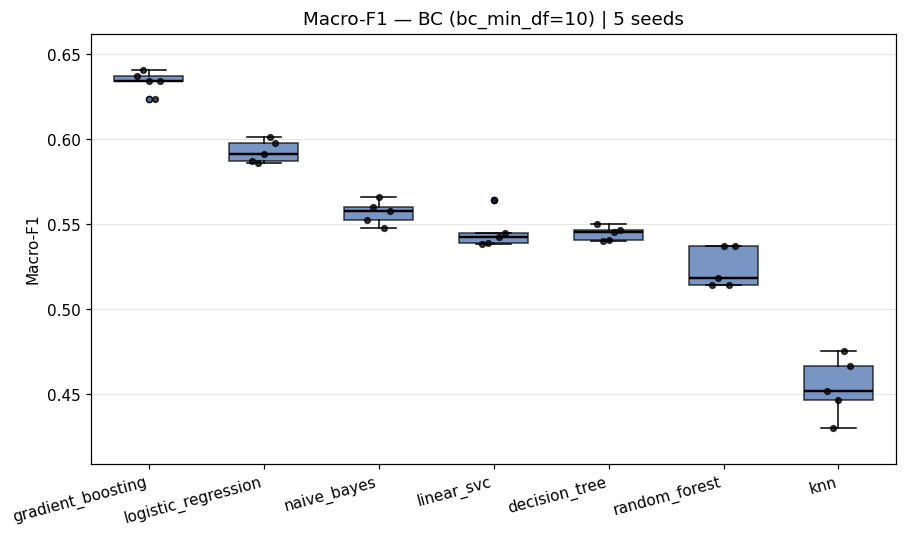
\includegraphics[width=0.42\linewidth]{figures/spot_check/macro_f1_boxplot_bc.png}
\hspace{0.04\linewidth}
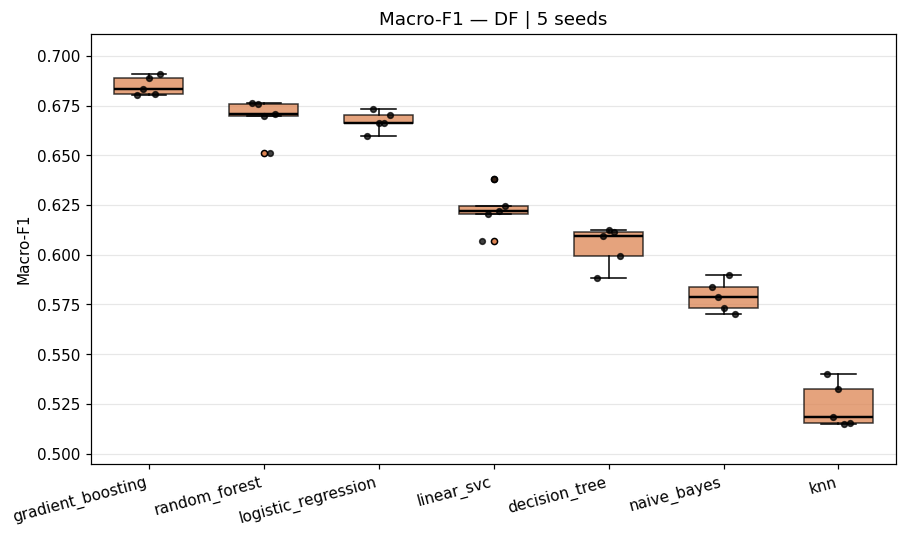
\includegraphics[width=0.42\linewidth]{figures/spot_check/macro_f1_boxplot_df.png}
\caption{Spot-checking macro-F1 per algorithm, across 5 seeds. Left: Bag of Cards. Right: Deck Features.}
\label{fig:spotcheck-boxplots}
\end{figure}

\end{document}
